\section{Overview}
\label{ch-introduction:sec:overview}

Today's society and its lifestyle are highly dependent on the continuous availability of energy.
More specifically: electrical energy, which has experienced the most significant increase in demand over the past decades.
One reasons behind this demand increase is due to the environmental aim to reduce green house gas emissions by 80\% by 2050.
Another reason is based on political agendas to reduce national dependence on fossil fuels like oil, coal and gas.
Therefore, governments incentivised and subsidised the uptake of Low Carbon Technologies (LCTs).
Ongoing electrification of heating and transport, as well as increased penetration of Distributed Generation (DG) are the results.
Whilst the electricity grid's infrastructure was initially constructed to deliver electricity in a unidirectional manner, it may no longer be able to support the current energy trends.
Conventional solutions are costly and disruptive network reinforcement.
Instead, electrical energy storage is proposed to support the network operation and mitigate or defer network reinforcement \cite{Manz2012, Kleinberg2014}.

The demand for electricity in the United Kingdom (UK) has increased significantly over the past century, and reports suggest that this trend is going to continue.
National Grid, one of the big UK network operators, published their Future Energy Scenarios (FES), highlighting the challenges that are yet to come \cite{FES2015}.
In this report, four scenarios have been identified, and National Grid explains them as follows (excerpts taken from FES \cite{FES2015}):

\begin{itemize}
	\item ``\textit{\textbf{Gone Green} is a world where green ambition is not restrained by financial limitations. New technologies are introduced and embraced by society, enabling all carbon and renewable targets to be met on time.}''
	\item ``\textit{\textbf{Slow Progression} is a world where slower economic growth restricts market conditions. Money that is available is spent focusing on low cost long-term solutions to achieve decarbonisation, albeit it later than the target dates.}''
	\item ``\textit{\textbf{No Progression} is a world focused on achieving security of supply at the lowest possible cost. With low economic growth, traditional sources of gas and electricity dominate, with little innovation affecting how we use energy.}''
	\item ``\textit{\textbf{Consumer Power} is a world of relative wealth, fast paced research and development and spending. Innovation is focused on meeting the needs of consumers, who focus on improving their quality of life.}''
\end{itemize}

\begin{figure}\centering
	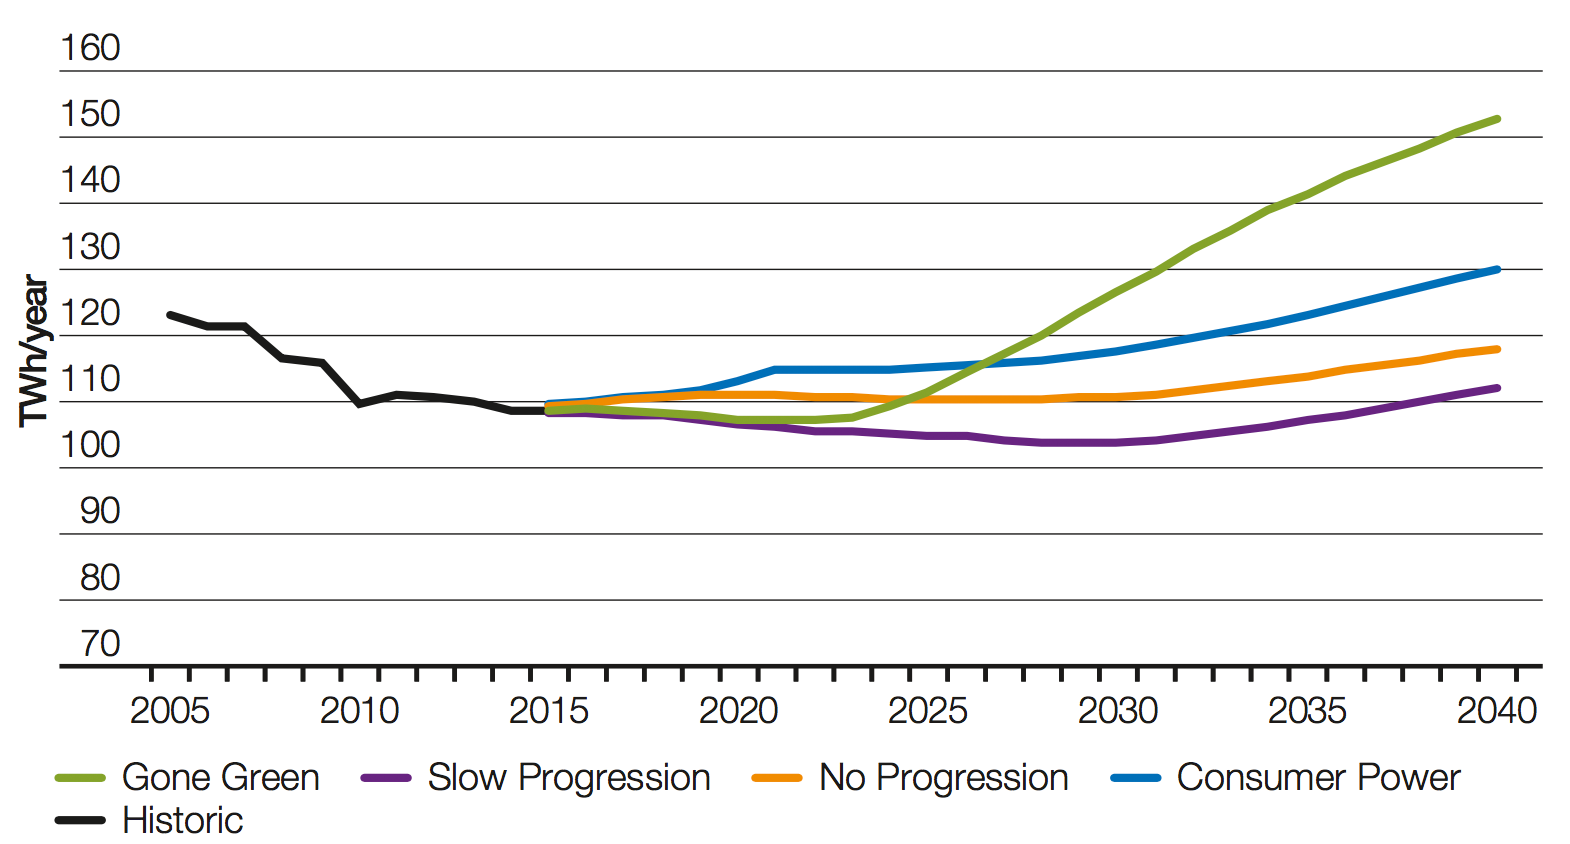
\includegraphics{_introduction/fig/electricity-demand-forecast}
	\caption{Annual residential demand for electricity from FES2016 \cite{FES2016}}
	\label{ch-introduction:fig:electricity-demand-forecast}
\end{figure}

In Figure \ref{ch-introduction:fig:electricity-demand-forecast} the UK's future residential electricity demand is plotted for each of the four scenarios.
Here, despite a subtle dip towards a new low in demand during 2025, all scenarios show an increase in energy demand after 2025.
Assuming that the UK is going to meet its environmental targets for 2050, National Grid's ``Gone Green'' scenario may be the most likely.

In this case the total demand for electricity is predicted to significantly increase.
This can be seen in Figure \ref{ch-introduction:fig:electricity-demand-change-forecast}, where the change in national energy demand is compared agains the current demand levels.
Here, increased industry efficiency is foreseen to outweigh its demand for electricity, which is shown by an initially negative change in demand.
Yet slower energy transitions in the private and commercial sector are foreseen to outweigh the industrial energy savings in 2025.
Also, the ongoing uptake of sustainable technology will result in a further rise in annual residential demand, by nearly 50TWh in 2036.
More than half of this residential demand, i.e. 27TWh, is expected to be caused by home charging of Electric Vehicles (EVs); which is the result of an expected 9.7 million EVs and Plug-in Hybrid EVs (PHEVs) being registered in the UK by 2040 \cite{DBER2008}.
This home charging will also have a significant impact on domestic peak power demnad.
In fact, it is expected to rise by as much as 6.5GW, predominantly because uncoordinated EV charging is feared to occur outside times of DG production \cite{FES2016}.

\begin{figure}\centering
	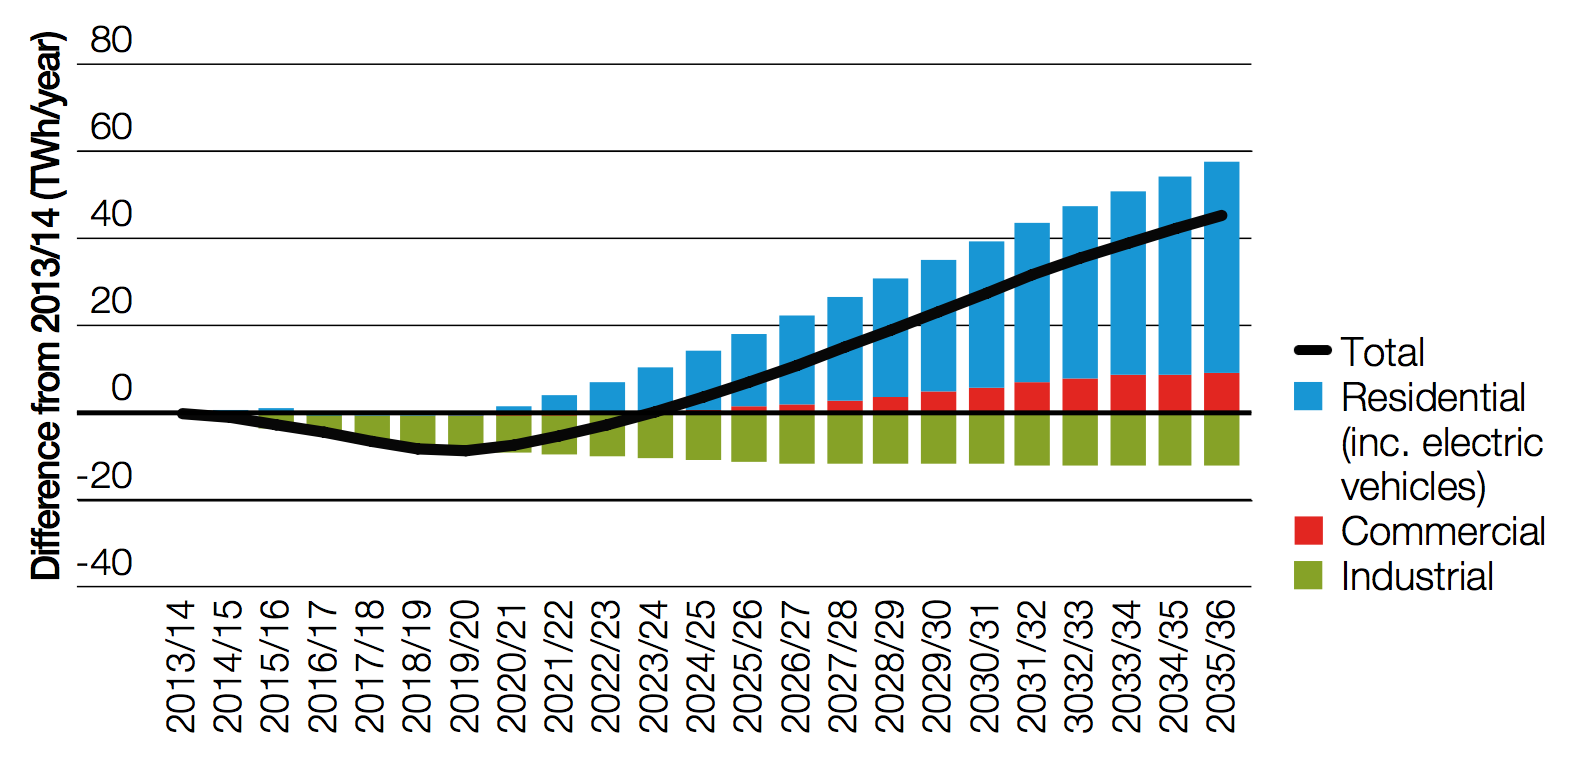
\includegraphics{_introduction/fig/electricity-demand-change-forecast}
	\caption{``Gone Green'' power demand comparison to 2013/14 by type (excluding losses) from FES2015 \cite{FES2015}}
	\label{ch-introduction:fig:electricity-demand-change-forecast}
\end{figure}

The corresponding impact of this increased peak demand varies across the grid.
For instance, the effect on the national transmission network's infrastructure is of little concern, since thermal limits are unlikely to be reached.
Nonetheless, balancing demand and supply and controlling the grid's operating frequency are still key aspects that need to be considered.
However, local power distribution networks are prone to thermal or voltage issues if peak demand is increased.
One solution may be the integration of Demand Side Response (DSM), where 
A study from 2010 shows that, as levels of EV and electric heating increase, equipment overloading becomes unavoidable unless devices are managed and coordinated intelligently \cite{Strbac2010}.
In fact, the study suggests that in a Business as Usual (BaU) case, all transformers in distribution networks will overload when EV penetration reaches a level of 75\%.
This was shown to be the case for both areas of high demand density (i.e. 2MVA/km$^2$) and low demand density (i.e. 0.5MVA/km$^2$).

In the UK, Distribution Network Operators (DNOs) are the owners of the power distribution networks.
Keeping this network within its operational constraints, e.g. preventing thermal overloads and voltage violations, used to be straight forward.
For traditional reasons, energy is acquired in half-hourly chunks, but with the increasing electricity demand and associated power variation, estimating half-hourly demand becomes more difficult, and responding to sudden demand spikes becomes more difficult.

As already mentioned, electrical energy storage, the main focus of this research, has been identified as an valid alternative to conventional network reinforcements.
With the aforementioned challenges in mind, the author of this thesis focuses on the improved control of this storage to support the operation of the Low-Voltage (LV) power distribution network.
More specifically, the question of how the important roles of electrical energy storage systems can be leveraged for both national and local benefits is addressed, and how their coordination is impacted by different external factors is researched.
The remainder of this chapter explains the traditional and upcoming role of energy storage in the grid.
Subsequent sections then introduce the \textit{New Thames Valley Vision} project, which is the funding body of the presented work, and the motivation and objectives.

%With the ongoing increase in demand for energy, power delivery networks that were constructed several decades ago are operated dangerously close to their capacity limits.
%Sociopolitical incentives to accelerate the uptake of Low-Carbon Technologies (LCTs) have commenced; e.g. to reduce the national green house gas emissions and reduce the dependency on oil, coal and gas.
%LCTs are twofold in nature.
%On the one hand Distributed Energy Resources (DERs), like wind or Photo Voltaic (PV) systems, can provide additional electrical energy, whilst the electrification of consumer appliances and transportation impose additional loads.
%For example, in 2012, due to government investment incentives like feed in tariffs or Renewable Obligation Certificates (ROCs), some European country's annual PV capacity increased by an astonishing 33GW \cite{Hockenos2013}.
%Furthermore, in just the UK, an uptake of 9.7 million EVs and Plug-in Hybrid Electric Vehicles (PHEV) is expected by 2040; requiring an additional 24TWh of energy \cite{DBER2008, FES2015}.
%Since this added generation and energy demand need not align in time, highly volatile demand fluctuations of large amplitude are the result.
%In fact, uncoordinated EV charging could impose an additional 6.5GW of demand onto the already stressed UK power grid \cite{FES2016}.
%To address the issue at its root cause, energy storage has been proposed \cite{Manz2012}.